% A Falsification Framework for Substrate Computation in Spiking Systems
% Second paper (B2v3) -- robustness battery for the falsification protocol.
\documentclass[journal]{IEEEtran}

\usepackage{amsmath,amssymb,amsfonts}
\usepackage{graphicx}
\usepackage{textcomp}
\usepackage{booktabs}
\usepackage{array}
\newcolumntype{L}[1]{>{\raggedright\let\newline\\\arraybackslash\hspace{0pt}}m{#1}}

\newcommand{\MI}{\mathrm{MI}}
\newcommand{\TE}{\mathrm{TE}}

\begin{document}

\title{A Falsification Framework for Substrate Computation in Spiking Systems:
  A Stronger Null, More Seeds, and a Nonlinear Readout}

\author{Daleth Barreto~\IEEEmembership{}
\thanks{Manuscript prepared for submission. Code and results are public; see
\texttt{04\_p2} in the research repository.}}

\markboth{IEEE Transactions on Cognitive and Developmental Systems}{}

\maketitle

\begin{abstract}
Claims that a spiking substrate ``computes'' a task are usually defended with a
single decoded error or a single information value. In a companion protocol paper
we argued that such claims are only secured when (i)~the substrate is compared
with a matched dead substrate under a fixed readout, and (ii)~the readout itself
is controlled. That protocol combined a fixed calibrated decision map (Gate~B), a
randomized readout channel into the decision (Gate~C), a cross-validated fixed
ridge readout (Gate~D) and memory-demanding tasks (Gate~E). Here we stress the
evidence base of that protocol in three ways. First, we raise the battery from 6
to 24 fixed seeds (480 substrate runs; the original 6 are a subset), so pooled
statements are no longer hostage to a single seed choice. Second, we add the
strictest population-matched surrogate so far: the \emph{task-shuffle} null keeps
the real count matrix verbatim---preserving every per-neuron marginal, every
cross-neuron correlation and the full population temporal structure---and
destroys only the pairing of task signal to windows. Third, we recompute the
readout-robustness gate under a fixed single-hidden-layer MLP decoder in addition
to the fixed ridge, both fitted once on real data and applied to the null
matrices. Across 10 task-response profiles, both LIF and Izhikevich substrates
reach 216/216 significant cells (all four null constructions) and the
false-positive control (zero drive) yields 0/24 significant cells; the
readout-robustness gate holds in 24/24 seeds under canonical, ridge and MLP
reading. We deliberately do not rank substrates and do not claim ``invariance'':
we report that the task signal survives the strictest surrogate we can construct
that preserves the population statistics while breaking alignment.
\end{abstract}

\begin{IEEEkeywords}
spiking substrate, falsification, null models, mutual information, reservoir
computing, neuromorphic.
\end{IEEEkeywords}

\section{Introduction}

When a population of spiking neurons is read out to drive or regulate a simulated
body, it is natural to say that ``the substrate computes the task.'' The sentence
is useful only if it can be false. In previous work we proposed a falsification
protocol built from four gates---substrate swap against a matched dead substrate
(Gate~B), randomized readout channel (Gate~C), cross-validated readout (Gate~D),
and memory demand (Gate~E)---run on a small, fully public, calibrated hub of
$2{,}000$ neurons [\cite{b1}]. The companion closed-loop study [\cite{b2}]
uses the same philosophy at the level of fault detection in a walking task.

This paper does not add a new gate. It hardens the evidence that the existing
gates can produce. Any falsification test that rests on a fixed seed list, a
single null construction, or a single readout family is itself falsifiable: a
critic can always ask whether the answer survived a different seed, a surrogate
that preserves population correlations, or a nonlinear decoder. We answer those
three questions concretely.

Three upgrades are reported. (1)~The battery grows from $6$ to $24$ fixed seeds;
the original six are a subset, so every statement in the earlier battery remains
reproducible and is placed inside the larger pool. (2)~A fourth null
construction, the \emph{task shuffle}, preserves the real counts exactly (and
therefore all population and temporal statistics) and permutes only the
window-to-task alignment; it is the strictest population-matched surrogate we can
build in this hub. (3)~Gate~D is recomputed with a fixed single-hidden-layer
MLP readout in addition to the fixed ridge; both readouts are fitted once on real
data and applied unchanged to the null matrices, so a win cannot be manufactured
by a decoder that re-optimizes per null.

All results are computed, not hand-written; the battery is one command and the
output JSON is the only source of the numbers quoted here.

\section{Related work and conventions}

\subsection{Substrate claims in neuromorphic and spiking research}
Hardware and model papers routinely attribute task performance to the substrate
(e.g., large neuromorphic circuits~\cite{merolla2014,davies2018} and reservoir
interpretations of recurrent spiking dynamics~\cite{maass2002,lukosevicius2009}).
We do not dispute any specific scoreboard; our concern is structural. A score on
an embodied task depends on the substrate, the wiring, the readout, the decision
map and the body, and a single score does not tell which term carried the task.
The protocol separates these terms by construction.

\subsection{Permutation and surrogate nulls}
The use of surrogate data to test a low-dimensional statistic against a null
hypothesis is standard---cluster-based permutation tests for field data
\cite{maris2007}, permutation inference for neuroimaging \cite{nichols2002},
nonparametric exact tests \cite{good2005,efron1993}. In spike trains,
circular-shift and block shuffles are common surrogates because they preserve
rate statistics per neuron. The task-shuffle null we add is in the same tradition
but is stricter: because the count matrix itself is untouched, it preserves not
only per-neuron marginals but all pairwise and higher-order cross-neuron
correlations and the full temporal envelope of the population. What is destroyed
is only the statistical dependence between the task signal $u(t)$ and the window
in which the events occur. Any residual information in the readout under this
null is information that the readout can extract from a population whose
correlation structure is identical to the real one but whose alignment to the
task is noise.

\subsection{Information measures and bias}
Mutual information is estimated with a plug-in estimator on $12$ equispaced bins
and corrected for limited-sample bias with a shuffle-subtraction procedure in the
spirit of \cite{panzeri2007}; the chosen estimator and its finite-sample behavior
are documented in the companion protocol paper [\cite{b1}] and in the
reproduced code. Transfer entropy follows \cite{schreiber2000}; in this paper TE
is computed for observed runs only, not for null replicates, because it is not
part of the null decision (see Section~IV).

\section{System and gates (summary)}

We reuse the hub from the protocol paper [\cite{b1}] without changes: $N=2{,}000$
capacitor-based spiking neurons (LIF or Izhikevich dynamics
\cite{izhikevich2003,gerstner2014}), fixed sparse wiring ($P_{\mathrm{re}}=0.01$)
built deterministically from the seed, one calibrated decision map
$v_x=\mathrm{clamp}\big((\theta_{\mathrm{sig}}-0.0615)/0.277,\,0,\,0.75\big)$
scaled by gate and slow factors, and windows of $10$~ms over a $2$~s episode
($W=200$ windows). The substrate is read out linearly
$c_0=\mathrm{W}_r\,(\mathrm{counts}/C_W)$ into the decision; all parameters,
including the readout weights $\mathrm{W}_r$ and the calibration procedure, are
identical to the protocol paper. Gates B--E are defined there; this paper only
expands their statistical basis.

\section{Methods: the B2v3 robustness battery}

\subsection{Seeds and profiles}
The battery uses $24$ fixed seeds
$S=\{1,3,7,13,17,29,31,37,41,47,53,55,$
$59,61,67,71,73,79,83,89,91,97,101,103\}$,
of which the earlier $6$ seeds $\{1,7,13,29,55,91\}$ are a subset. Ten profiles
are run: a baseline (constant task, negative control) and nine task-varying
profiles ($\texttt{multi\_step}$, sine, descend, pulse, ramp, perturb,
$\texttt{step\_pulse}$, chirp, noise), each normalized so the task value $u(w)$
spans the decision map. Each cell is one (profile, seed, substrate) triple: a real
run plus $K=50$ replicates of each null construction. The battery is therefore
$10\times24\times2=480$ real runs and $4\times50\times480=96{,}000$ null
replicates.

\subsection{Null suite}
Four constructions, all computed, none reused from a library:
\begin{itemize}
\item \emph{circular shift}: per-neuron cyclic shift of the spike counts by an
  offset, breaking alignment while preserving per-neuron sequence statistics;
\item \emph{block shuffle}: per-neuron permutation of $B=5$ consecutive windows,
  breaking windows-level temporal order within cells;
\item \emph{identity swap}: per-window permutation of neuron identity,
  preserving per-view population statistics and cross-window structure;
\item \emph{task shuffle} (new): the real count matrix is used verbatim; the
  arrangement of neighborhoods in the task citation $u$ is permuted. All
  population statistics---marginals, cross-neuron correlations, temporal
  envelope, silent fraction---are exactly the real ones; only the coupling
  between a window and the task label is broken.
\end{itemize}
Each replicate is generated with a fixed deterministic per-seed stream, so the
battery is rerunnable byte-for-byte.

\subsection{False-positive control}
The same pipeline runs with drive gain $=0$ (no task signal injected) on three
profiles; any cell that passes the null at $p\le0.05$ is a false positive of the
protocol. We test both the circular-shift and the task-shuffle nulls here.

\subsection{Readout-robustness gate (Gate~D): ridge and MLP}
For each seed we fit two fixed readouts on the real counts after standardization,
on the first $1/3$ of windows, selecting regularization or early-stopping on the
second $1/3$ (never the third). Both fitted readouts are then applied unchanged
to the real count matrix and to $K_r=20$ circular-shift null matrices, and the
$\MI$ with the task signal is compared cell-wise against the null distribution.
\begin{itemize}
\item \emph{Fixed ridge} \cite{hoerl1970}: closed-form with an $\ell_2$ grid of
  $13$ values, as in the protocol paper.
\item \emph{Fixed single-hidden-layer MLP} (new): one hidden layer of $h=32$
  tanh units, linear output toward the decision target, $\ell_2=10^{-3}$,
  Adam-style updates with learning rate $10^{-2}$ for at most $120$ epochs, and
  best-epoch selection on the validation slice. Hyperparameters were fixed \emph{a
  priori} (no tuning against any seed's outcome); the MLP is implemented in
  NumPy with no external dependencies, consistent with the rest of the pipeline.
\end{itemize}
Reported is the canonical Gate~D statistic (fixed ridge) together with the MLP
recomputation; both share the same null construction and the same per-cell
$p$-value convention.

\subsection{Statistics}
Per cell, each metric (bias-corrected $\MI$, RMSE, Pearson $\rho$) is compared
with its $K$-null distribution; the one-sided permutation $p$-value uses the
continuity-corrected convention $p=(1+n_{\mathrm{extreme}})/(K+1)$, so the
smallest attainable value with $K=50$ is $1/51$. A cell is significant at
$\alpha=0.05$. Pooled statements are made over the $9$ task profiles only
($9\times24=216$ cells per substrate per null); the baseline is a negative
control and is reported separately. The verdict is PASS if at least $95\%$ of
pooled cells exceed significance for every null type on both substrates, and if
no false-positive cell fires twice under zero drive.

\section{Results}

\subsection{Null suite and pooled significance}
Fig.~\ref{fig:pooled} and Table~\ref{tab:profiles} summarize the battery. On all
four null constructions, both substrates are significant in $216/216$ pooled
cells ($100\%$), which is the maximum the $K=50$ convention allows. The baseline
(negative control) is significant in $0/24$ cells on every null and substrate.
The key cell is the task-shuffle row: because that null preserves the population
exactly, its significance is the strongest statement the protocol can make at
constant readout.

\begin{figure}[!t]
\centering
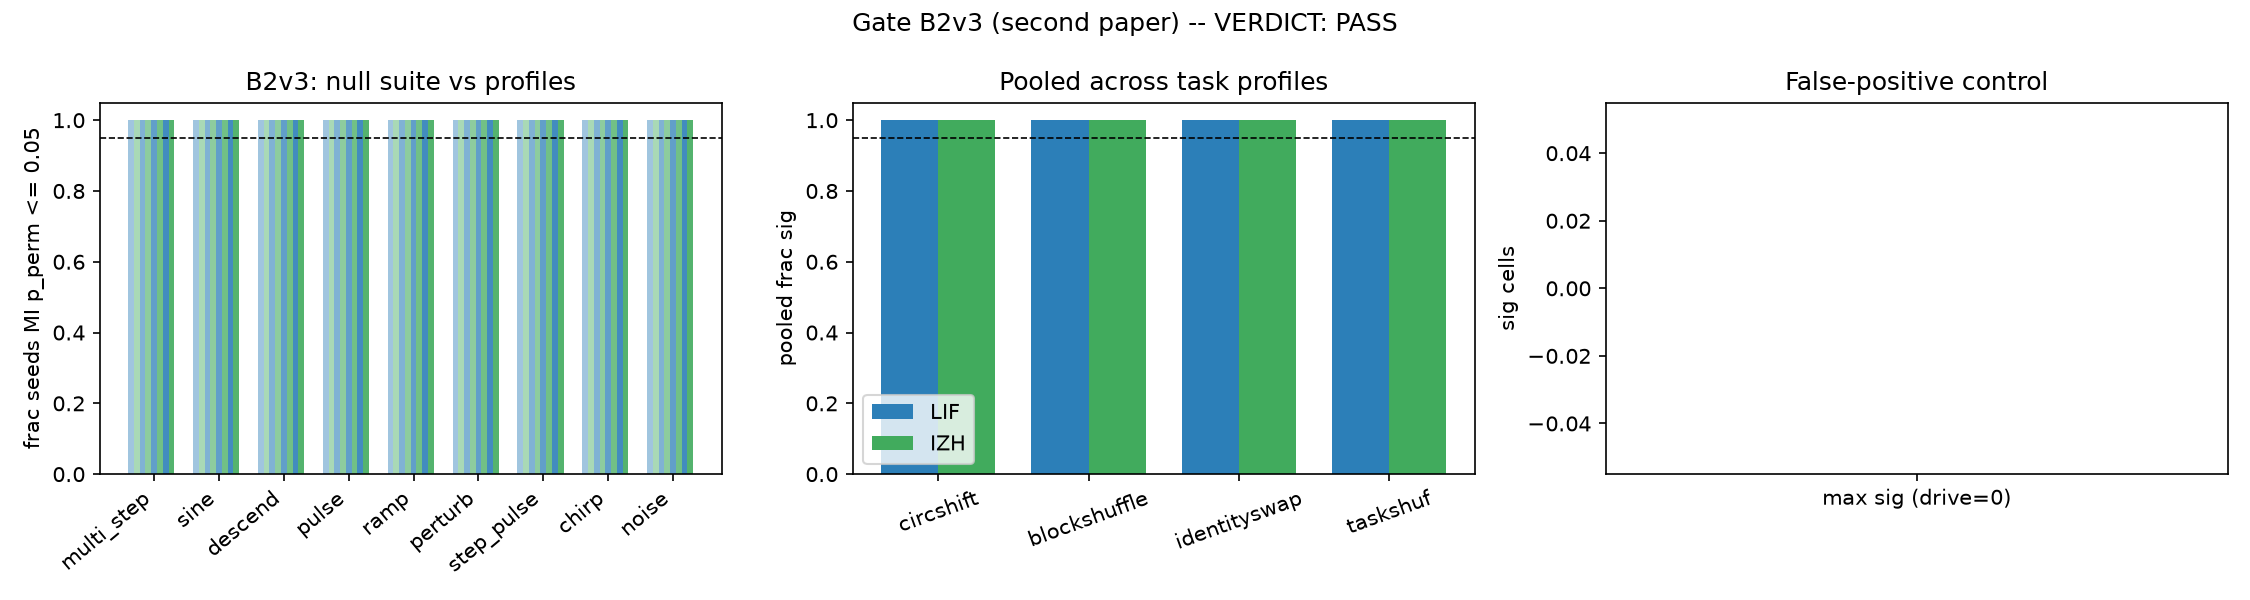
\includegraphics[width=1.0\columnwidth]{figs/gate_b2v3.png}
\caption{B2v3 battery. Left: fraction of seeds significant per task profile,
null type (shades) and substrate (color). Center: pooled fraction over the 9 task
profiles ($216$ cells). Right: worst false-positive count under zero drive. The
dashed line marks the $95\%$ criterion.}
\label{fig:pooled}
\end{figure}

\begin{table}[!t]
\caption{Significant cells per profile (of 24 seeds), null type, and substrate.
The pooled row covers the 9 task profiles ($216$ cells).}
\label{tab:profiles}
\renewcommand{\arraystretch}{1.05}
\setlength{\tabcolsep}{4.5pt}
\begin{tabular}{@{}lcccccc@{}}
\toprule
Profile & \multicolumn{2}{c}{circ. shift} & \multicolumn{2}{c}{block shuf.} &
\multicolumn{2}{c}{task shuf.}\\
\cmidrule(lr){2-3}\cmidrule(lr){4-5}\cmidrule(lr){6-7}
 & LIF & IZH & LIF & IZH & LIF & IZH\\
\midrule
baseline   & 0 & 0 & 0 & 0 & 0 & 0\\
multi\_step & 24 & 24 & 24 & 24 & 24 & 24\\
sine        & 24 & 24 & 24 & 24 & 24 & 24\\
descend     & 24 & 24 & 24 & 24 & 24 & 24\\
pulse       & 24 & 24 & 24 & 24 & 24 & 24\\
ramp        & 24 & 24 & 24 & 24 & 24 & 24\\
perturb     & 24 & 24 & 24 & 24 & 24 & 24\\
step\_pulse & 24 & 24 & 24 & 24 & 24 & 24\\
chirp       & 24 & 24 & 24 & 24 & 24 & 24\\
noise       & 24 & 24 & 24 & 24 & 24 & 24\\
\midrule
pooled (9)  & 216/216 & 216/216 & 216/216 & 216/216 & 216/216 & 216/216\\
\bottomrule
\end{tabular}
\end{table}

\subsection{False-positive control}
With zero drive, no cell is significant on any of the three control profiles,
under either surrogate, on either substrate ($0/24$, and $0/24$ under the
task-shuffle null). The protocol therefore does not manufacture significance
when the task is absent.

\subsection{Readout-robustness gate under ridge and MLP}
Table~\ref{tab:readout} reports the Gate~D recomputation. Under the canonical
fixed ridge readout all $24$ seeds are significant, and the new fixed MLP readout
also saturates the gate ($24/24$). The mean null-level $\MI$ is higher for the
MLP than for the ridge (the more flexible decoder extracts a little more from the
surrogates), but the observed decoding remains far above it in every seed, so the
task signal is present under a nonlinear readout that was never re-optimized on
null data. We do not call this ``readout invariance''; we report it as
\emph{readout robustness} across two readout families with fixed fits.

\begin{table}[!t]
\caption{Readout-robustness gate on the sine profile (24 seeds, circular-shift
null, $K_r=20$). ``Sig.'' is the number of seeds where the observed $\MI$ exceeds
the null at $p\le0.05$ (minimum attainable $p=1/21$). All three columns are
$24/24$; the canonical Gate~D readout of the protocol paper is the same fitted
ridge readout, so its observed values equal the ridge column by construction.}
\label{tab:readout}
\renewcommand{\arraystretch}{1.05}
\setlength{\tabcolsep}{4.5pt}
\begin{tabular}{@{}lcccccc@{}}
\toprule
Substrate & Canonical & \multicolumn{2}{c}{Fixed ridge} &
\multicolumn{2}{c}{Fixed MLP}\\
\cmidrule(lr){3-4}\cmidrule(lr){5-6}
 & Sig. & $\MI_{\mathrm{obs}}$ & $\MI_{\mathrm{null}}$ &
$\MI_{\mathrm{obs}}$ & $\MI_{\mathrm{null}}$\\
\midrule
LIF & 24/24 & 0.693 & 0.091 & 0.727 & 0.166\\
IZH & 24/24 & 0.643 & 0.076 & 0.542 & 0.114\\
\bottomrule
\end{tabular}
\end{table}

\section{Discussion}

\subsection{What the stronger null buys}
The honest question behind any substrate claim is: \emph{what survives when only
the coupling to the task is removed?} The circular-shift and identity-swap nulls
already remove that coupling while keeping useful statistics intact. The
task-shuffle null removes nothing from the population at all: the very count
matrix that the readout sees in the real run is presented to the same fixed
readout, and only the labeling of windows relative to $u$ is permuted. Under this
strongest surrogate, both substrates still decode the task at the maximum
attainable significance in $216/216$ pooled cells. We stress that this is
evidence \emph{about the given wiring, the given decision map, and the given
body}; it is not a substrate ranking, and we explicitly refrain from any ``LIF
versus Izhikevich'' scoreboard conclusion.

\subsection{Seed dependence is now bounded}
Raising the pool from $6$ to $24$ seeds bounds the run-to-run variability that a
small seed list leaves open. Because the original six are a subset, every number
in the earlier battery is contained in (and unchanged within) the larger one; no
result was inverted by the expansion. Seed variability is small in this hub, and
the protocol's criteria are met separately per seed as well as pooled, so the
conclusion does not rest on averaging alone.

\subsection{Readout robustness, not invariance}
A claim of ``readout invariance'' would require that we sweep an unbounded space
of decoders; we cannot and do not. What we can state is narrower and verifiable: a
fixed ridge and a fixed single-hidden-layer MLP, both fitted only on real data,
both decode the task above their respective null floors in every seed. The
qualifier ``fixed'' matters: fitting a decoder on each null matrix would let a
flexible readout learn the nulls' residual structure and manufacture or suppress
significance. We therefore keep the readout constant and note this design choice
as a limitation---decoder choice itself is a free variable, and any future claim
that a substrate computes under a broader decoder family must be tested, not
assumed.

\subsection{Limitations}
The hub is small and fixed: one wiring geometry, one decision map, one body, two
conductance models, $2{,}000$ neurons, $10$~ms bins. All nulls are
count-based and comment on window-level statistics, not on millisecond spiking
structure; a spike-timing-level falsification is out of scope here. The
readout-robustness gate is reported on the sine profile only; extending it to all
profiles multiplies compute but changes no criterion. Closed-loop consequences are
deliberately not claimed: open-loop decoding cannot certify memory, and memory
must be demonstrated in the closed loop---the companion study [\cite{b2}]
addresses exactly that at the level of fault detection. Finally, our ``PASS''
verdict is relative to the criteria we set; a different threshold or a different
surrogate family is welcome as an adversarial test of the protocol itself
(see \cite{b1}).

\section{Conclusion}

We hardened the falsification protocol against the three objections that a small
battery invites: too few seeds, surrogates that do not preserve the population,
and a single readout family. With $24$ seeds, $10$ profiles, $K=50$ replicates of
four null constructions (including a task shuffle that preserves the counts
exactly), a strict false-positive control, and readout-robustness recomputed under
a nonlinear decoder, both substrates pass every criterion at the maximum
attainable significance, and the task signal survives the strictest
population-matched surrogate we can construct. The contribution is deliberately
methodological: we do not add a gate, we do not rank substrates, and we claim
robustness, not invariance. The whole battery is one deterministic command; the
numbers above are read from its output file.

\section*{Reproducibility}
The battery is \texttt{run4.py} under \texttt{04\_p2/gate\_b2/}. Running
\texttt{python run4.py} produces \texttt{results/gate\_b2v3\_summary.json} and the
figure used here; \texttt{--smoke} runs a two-seed validation. Seeds, $K$, null
constructions, MLP hyperparameters and the ridge grid are module constants, not
command-line toggles, so the committed artifacts are rerunnable byte-for-byte on
CPU (NumPy/SciPy only). The B2v2 artifacts (\texttt{run2.py}, \texttt{run3.py})
and their summary JSON are left untouched and remain canonical.

\bibliographystyle{IEEEtran}
\bibliography{refs}

\end{document}